\section{Flow over a cylinder}
\label{sec_cylinder}  

In this section, a flow over a cylinder is solved with {\psiboil}.
The flow is two-dimensional and isothermal and occurs at relatively low
Reynold number ($Re$). This problem will tech you how to define boundary
conditions for some parts of the boundary and is also a first fluid flow 
solver in this tutorial.

The geometry and boundary conditions are shown in~Fig.~\ref{fig_cylinder},
and dimensions are specified as following: $L=2.2$, $H=0.41$, and $W=H/2$.
Cylinder diameter is set to~$D=0.1$. Distance of cylinder axis to lower
corner of the inlet is~$h=0.2$, meaning the cylinder is not placed 
symmetrically in the problem domain. It is intentionally so, to promote
earlier transition to a vortex shedding regime. 

%------------%
%            %
%  Cylinder  %
%            %
%------------%
\begin{figure}[ht]
  \centering
  \setlength{\unitlength}{1mm}
  \begin{picture}(100, 43)(0,0)
    \thickbox{100}{ 43}
    \put(0,0){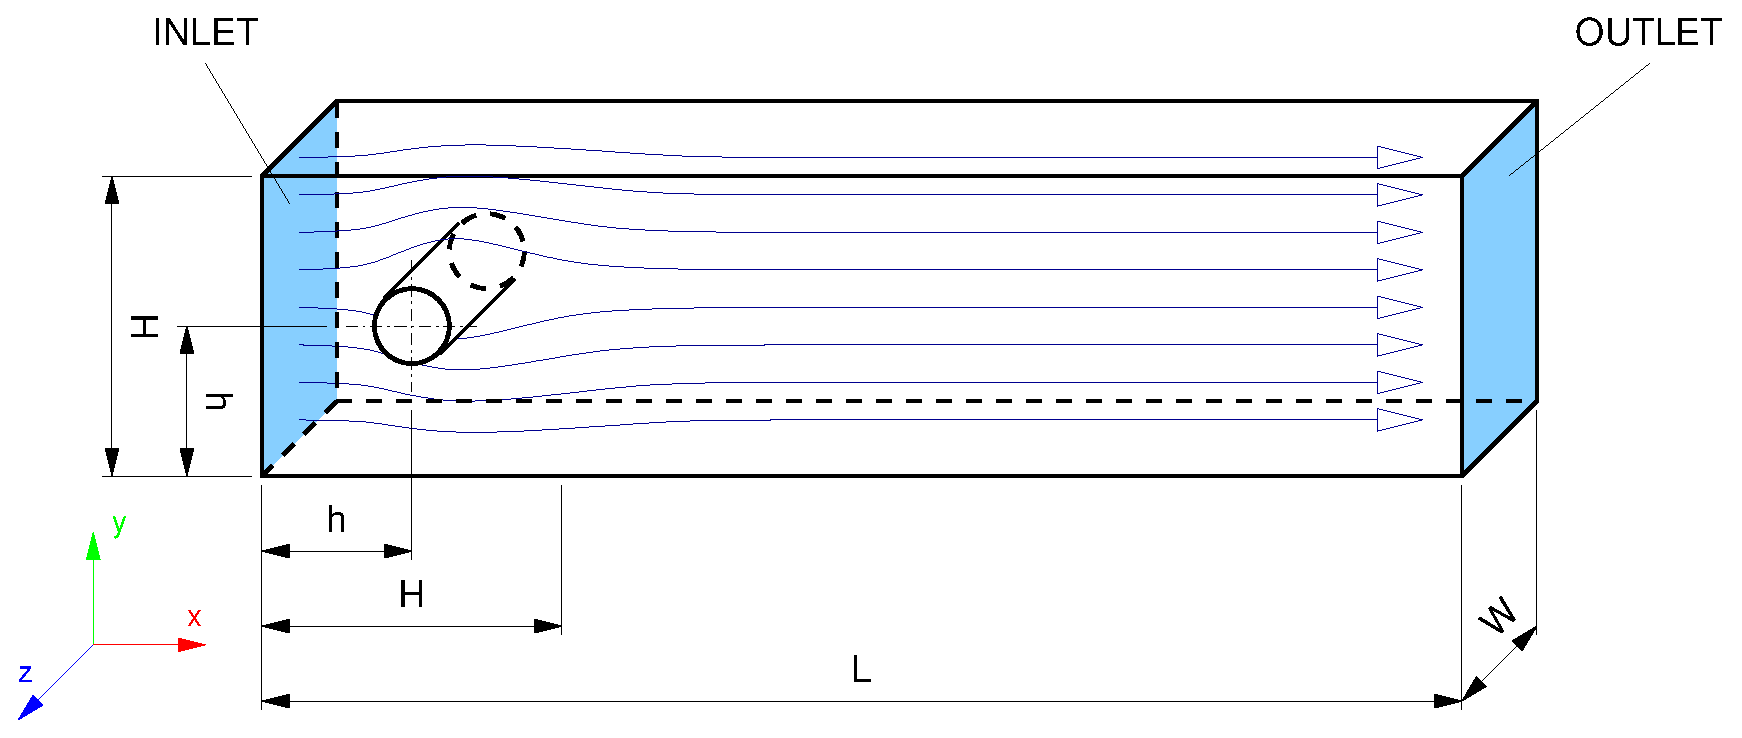
\includegraphics[scale=0.35]{Figures/09-01-domain.eps}}
  \end{picture}
  \caption{Geometry, boundary conditions and basic topology for the
           flow over a cylinder.}
  \label{fig_cylinder}
\end{figure}

Parabolic velocity profile is specified at the inlet according to the equation:
%
\be
  u = 4 \cdot U_m \cdot y \cdot (H-y)/H^2
\ee
%
where~$U_m$ is maximum inlet velocity equal to~1.5.

The program which solves this problem is stored under name {\tt 09-01-main.cpp}
and will be outlined in the rest of this chapter. However, different program
units, as outlined in Ch.~\ref{chap_structure}, will be introduced in separate
sub-sections. For the sake of shortness, some program comments will be skipped. 

Domain dimensions, as well as resolutions, are defined as constants outside
the body of the main function as:
%
{\small \begin{verbatim}
      3 /* dimensions */
      4 const real H  = 0.41;
      5 const real L  = 2.2;
      6
      7 /* resolutions */
      8 const int NY =  64;
      9 const int NX1 = NY;
     10 const int NX2 = NY;
     11 const int NZ  = NY/8;
\end{verbatim}}
%
The grid will be uniform in $y$ and $z$ (normal and span-wise), but
not in $x$ (stream-wise) direction. That is why we introduce two variables
for resolution in $x$, namely {\tt NX1} and {\tt NX2}.

\subsection{Domain}

IB, in this case cylinder, is defined in line 23:
%
{\small \begin{verbatim}
     23   Body cyl("09-01-cylinder.stl");
\end{verbatim}}
%
Clearly, cylinder is defined in STL format in file {\tt 09-01-cylinder.stl}, 
which must be present in the running directory. 

Grids are defined with the following lines:
%
{\small \begin{verbatim}
     28   Grid1D gz ( Range<real>(-H/4, H/4), NZ,  Periodic::yes());
     29   Grid1D gy ( Range<real>( 0.0, H  ), NY,  Periodic::no());
     30   Grid1D gx1( Range<real>( 0.0, H  ), NX1, Periodic::no());
     31   const real dx = H/(real)NY;
     32   Grid1D gx2( Range<real>( H,   L  ), Range<real>(dx, 8.0*dx), NX2, Periodic::no());
     33   Grid1D gx( gx1, gx2, Periodic::no());
\end{verbatim}}
%
No stretching is used in normal and span-wise ($y$ and $z$) direction. 
Span-wise direction is defined to be periodic. Grid in stream-wise~($x$)
direction is created from two parts: a {\em uniform} part, spanning 
from~$x=0$ to~$x=H$, created in line~30 as {\tt gx1} and a {\em non-uniform} 
one, spanning from~$x=H$ to~$x=L$, created in line~32 as~{\tt gx2}. 
The size of first cell in {\tt gx2} is set to be {\tt dx}, which corresponds
to cell size in~{\tt gx1}. Final grid in~$x$ direction is created in line~33
as a union of~{\tt gx1} and~{gx2}.

Once the IB and grids are defined, domain is created in line~38
with:
%
{\small \begin{verbatim}
     38   Domain d(gx, gy, gz, &cyl);
\end{verbatim}}

%--------%
%        %
%  Mesh  %
%        %
%--------%
\begin{figure}[h!]
  \centering
  \setlength{\unitlength}{1mm}
  \begin{picture}(140, 32)(0,0)
    \thickbox{140}{ 32}
    \put(0,-45){\includegraphics[scale=0.60]{Figures/09-01-mesh.eps}}
  \end{picture}
  \caption{Computational grid for the flow around a cylinder.}
  \label{fig_cylinder_mesh}
\end{figure}

\subsection{Field variables}

Now we have reached the second logical unit of the program, which defines
field variables. For this case, we have velocity and momentum forces
as {\tt Vector}'s and pressure and it's source as {\tt Scalars}, defined
in lines~40 and~41:
%
{\small \begin{verbatim}
     43   Vector uvw(d), xyz(d); /* velocity and its source */
     44   Scalar p  (d), f  (d); /* pressure and its source */
\end{verbatim}}
%
This is followed by the definition of boundary conditions. Since {\tt Vector}s
have three components, boundary conditions have to be assigned through a loop
browsing through them, as it is done in lines~49--57:
%
{\small \begin{verbatim}
     49   for_m(m) {
     50     uvw.bc(m).add( BndCnd( Dir::imin(), BndType::inlet(),
     51                    "4.0*1.5*y*(0.41-y)/0.41^2", "0.0", "0.0") );
     52     uvw.bc(m).add( BndCnd( Dir::imax(), BndType::outlet() ) );
     53     uvw.bc(m).add( BndCnd( Dir::jmin(), BndType::wall() ) );
     54     uvw.bc(m).add( BndCnd( Dir::jmax(), BndType::wall() ) );
     55     uvw.bc(m).add( BndCnd( Dir::kmin(), BndType::periodic() ) );
     56     uvw.bc(m).add( BndCnd( Dir::kmax(), BndType::periodic() ) );
     57   }
\end{verbatim}}
%
Browsing is performed with macro {\tt for\_m}, defined in {\tt Field/Vector/vector\_browsing.h}.
Variable representing vector component is defined as {\tt m} throughout {\psiboil}. It is a
ravioli object of type~{\tt Comp}.
Member function for defining boundary conditions for {\tt Vector}s defined from the one for
scalars (introduced in~Sec.~\ref{sub_sec_bc}) because it also has to provide the component for
which this boundary condition applies, i.e.\ the syntax of the member function is:
%
{\small \begin{verbatim}
     Vector::bc(Comp m).add( BndCnd & );
\end{verbatim}}
%
In lines~50--51 inlet is defined ({\tt BndType::inlet()}) at inlet plane ({\tt Dir::imin()}).
For velocity inlet, three values must be specified, one for each component. They are
defined in line~55 as: {\tt "4.0*1.5*y*(0.41-y)/0.41\^2"}, {\tt "0.0"} and {\tt "0.0"}.
{\psiboil} supports analytically prescribed boundary conditions, as long they are
functions of $x$, $y$ and $z$. For velocity outlet, as well as for wall and periodic
conditions, no values need to be specified, as shown in lines~52--56.

Boundary conditions for the pressure, when solved with the projection method, should
be $\frac{\p p}{\p n} = 0$ on all boundaries where velocities are known.
In this case, this are all, except the ones at periodic ones. All boundary conditions
for pressure are defined in lines~62--67:
%
{\small \begin{verbatim}
     59   p.bc().add( BndCnd( Dir::imin(), BndType::neumann() ) );
     60   p.bc().add( BndCnd( Dir::imax(), BndType::neumann() ) );
     61   p.bc().add( BndCnd( Dir::jmin(), BndType::neumann() ) );
     62   p.bc().add( BndCnd( Dir::jmax(), BndType::neumann() ) );
     63   p.bc().add( BndCnd( Dir::kmin(), BndType::periodic() ) );
     64   p.bc().add( BndCnd( Dir::kmax(), BndType::periodic() ) );
\end{verbatim}}
%
Note that boundary conditions have been defined for both variables at all 
boundary planes. No patch remained undefined. That is a {\em rule}. 
{\psiboil} {\em does not} support {\em default} boundary conditions for 
any variable. 

\subsection{Physical properties, time and solver}

We have reached the third unit (according to standard {\psiboil} program
layout outlined in~Fig.~\ref{fig_structure}, which defines physical 
properties ({\tt Matter}), simulation time ({\tt Times}) and linear
solver ({\tt Krylov}). In this program, the third unit looks like:
%
{\small \begin{verbatim}
     69   Matter fluid(d);
     70
     71   fluid.mu(0.001);
     72
     73   Times time(10000, dx/8.0);
     74
     75   Krylov * solver = new CG(d, Prec::di());
\end{verbatim}}
%
New substance is created with the name {\tt fluid} in line~69, and its
dynamic viscosity has been set to $0.001$ in line~71. Simulation time
is represented with object {\tt time}, created with number of time
steps equal to~10000 and time step equal to $\Delta t=dx/8$
The value of time step is calculated from the requirement 
that Courant-Friedrich-Levy (CFL) number is around $\frac{1}{4}$ during the
simulation\footnote{Keep in mind that maximum value of inlet velocity is~1.5
and that $\Delta x = dx$}. Time variable may be defined in
other ways. Instead of number of time steps and the time step value,
we could have defined total simulation time and number of time steps.
The details of these, and other possible definitions, take a look at
{\tt Src/Ravioli/times.h}.

\subsection{Transport equations}

Two transport equations are defined in the fourth unit, one for momentum
transport~(\ref{eq_momentum_2}) and one for pressure-Poisson~(\ref{eq_pressure_2}):
%
{\small \begin{verbatim}
     80   Pressure pr(p, f, uvw, time, solver, &fluid);
     81   Momentum ns( uvw, xyz, time, solver, &fluid);
\end{verbatim}}
%
Attributes sent to {\tt Pressure} constructor are the pressure {\tt p}
and its source {\tt f}, used for storing the right hand side 
of~Eq.~\ref{eq_pressure_2}, which is computed from velocity~{\tt uvw},
sent as a third parameter. {\tt Momentum} constructor takes velocity
field {\tt uvw} and its forces {\tt xyz} as parameters. Both 
{\tt Pressure} and {\tt Momentum} constructor need variable defining
simulation time, solver and substance, represented in lines~80
and~81 as objects {\tt time}, {\tt solver} and {\tt fluid}.

\subsection{Preparation for the time-loop}

The fifth unit contains only one line:
%
{\small \begin{verbatim}
     83   AC multigrid( &pr );
\end{verbatim}}
%
which creates a multigrid solver for the {\tt Pressure p}. When solving
transient transport equations, it is sound to create a multigrid solver
for pressure only. Transported variables (momentum, enthalpy, \dots)
give well-conditioned systems which can be solved with {\tt Krylov}
solver only. Even more, multigrid solver {\em can not} be defined
for momentum equations, since they change their resolution due to
staggered arrangement of variables. No variable needs initialization for 
this problem.

This program features modest $Re$, but for this geometry, it should yield
and oscillatory solution, {\em i.e.} it should lead to  vortex shedding.
Therefore, it would be convenient if {\psiboil} was printing the value 
of certain variable at a point in the domain during the simulation to check
whether an oscillatory solution has been reached, or to check the frequency
of oscillations, etc. There is a class which does just that. It is 
called~{\tt Location} and is defined in {\tt Src/Monitor/Location}.
Here, we define a {\tt Location} as:
%
{\small \begin{verbatim}
     85   Location loc("monitor", d, NX1, NY/2, NZ/2);
\end{verbatim}}
%
It creates {\tt Location loc}, called {\tt "monitor"}, in the {\tt Domain d},
at logical coordinates ($i$, $j$ and $k$) equal to {\tt NX1}, {\tt NY/2}, 
and {\tt NZ/2}. That {\tt Location} will be placed midway between the walls
in the region where uniform~({\tt gx1}) and non-uniform~({\tt gx2}) grids
meet. It's usage is explained below. 

\subsection{The time-loop}

Finally, we reach the time loop of the program, reading:
%
{\small \begin{verbatim}
     90   for(time.start(); time.end(); time.increase()) {
     91
     92     boil::oout << "##################" << boil::endl;
     93     boil::oout << "#                 " << boil::endl;
     94     boil::oout << "# TIME:      " << time.current_time() << boil::endl;
     95     boil::oout << "#                 " << boil::endl;
     96     boil::oout << "# TIME STEP: " << time.current_step() << boil::endl;
     97     boil::oout << "#                 " << boil::endl;
     98     boil::oout << "##################" << boil::endl;
     99
    100     ns.cfl_max();
    101
    102     ns.new_time_step();
    103
    104     ns.solve(ResRat(1e-2));
    105
    106     p = 0.0;
    107
    108     multigrid.vcycle(ResRat(1e-2));
    109
    110     ns.project(p);
    111
    112     loc.print(uvw, Comp::v());
    113
    114     if( time.current_step() % 100 == 0)
    115       boil::plot->plot(uvw,  p, "uvw,p",  time.current_step());
    116   }
\end{verbatim}}
%
This loop embodies an implementation of fractional step algorithm in {\psiboil}.
In line~90 you can see how can variable {\tt time} be used to cycle through time.
It's member functions {\tt Times::start()}, {\tt Times::end()} and {\tt Times::increase()}
serve as parts of {\tt C++}'s {\tt for} loop. The advantage is that this loop 
remains the same, no matter how the variable {\tt time} was defined. 
Two additional {\tt Times}' member functions are used to plot current simulation
time and time step in lines~94 and~96. 

Line~100 calls {\tt Momentum}'s member function {\tt Momentum::cfl\_max} which computes
and prints the value of CFL number. Is it not necessary to call it, but it may serve
as a good indication why a certain simulation crashed\footnote{If CFL numbers gradually
increase, and gradually reach values higher than 0.5, simulation will be inaccurate
and will probably crash due to a too high time step.}. If CFL is too low, on the
other hand, we are wasting a lot of computational time. As a {\em rule of thumb}, optimum
CFL is in the range from $0.35 - 0.4$. 

Preparation for the new time step (which involves computation of terms with 
superscript~$n-1$ and~$n-2$ in Eq.~\ref{eq_semi}) are performed at line~102. That
is followed by it's solution at line~104. At that point, we have tentative 
velocity ($\uvw^\s$). 

In line~108, {\psiboil} uses the tentative velocity field to compute the right hand
side of~Eq.\ref{eq_pressure_2} and solve it to get the new pressure field. For unsteady
simulations, convergence of the multigrid solution for the pressure usually improves
if pressure is initialized to zero. It is performed in line~106. 

This pressure field is used to {\em project} tentative velocity ($\uvw^\s$)
into a new ($n$) divergence-free field~($\uvw^n$). This closes the fractional
step algorithm for one time step, and the new one can start. 

Line~112 shows how can an object of type {\tt Location} be conveniently used to
monitor the computed values. It prints the value of the argument (here {\tt Vector}
and it's component) at position defined in line~91, during the construction of
{\tt Location}. 

The programs plots the results (for velocities and pressure) every~100$^{th}$ from
lines~114 and~115.

\subsection{Running the program}  

Compile and run this program. Run it with:
%
\begin{verbatim}
> ./Boil > out &
\end{verbatim}
%
to store the terminal output to file {\tt "out"}. This simulation might take few hours
to finish. If you would like to check the progress during the run, issue the
command:
%
\begin{verbatim}
> tail -100f out
\end{verbatim}
%
As an example, output for time step~20 looks like:
%
{\small \begin{verbatim}
##################
#
# TIME:      0.0152148
#
# TIME STEP: 20
#
##################
cfl max = 0.230888 in direction u  at: 0.192187 0.265859 -0.0384375
u, residual = 6.87374e-07, ratio = 0.000281587
v, residual = 4.13061e-07, ratio = 0.000270693
w, residual = 2.03872e-08, ratio = 0.000250742
FILE: momentum_scale_out.cpp, LINE: 24, volf_in = 0.0840603
FILE: momentum_scale_out.cpp, LINE: 77, ratio = 1.00061
@get_src; err sou = 0.471205 -0.0399352
Initial  res = 0.00387017
Cycle 1; res = 0.000186533
Cycle 2; res = 8.59826e-05
Cycle 3; res = 2.87255e-05
Converged in 3 cycles!
monitor: -0.00159419
\end{verbatim}}
%
The lines beginning with a {\tt \#} only mark the beginning of a time step.
CFL is printed right after that. The following two lines show the result
of solving of momentum equations. {\tt residual} is the residual of 
the solving procedure, and {\tt ratio} shows the level of reduction of
residuals in the solvers. (For example, for {\tt w}, residuals were
reduced by roughly $4000$ times).
%
The following two lines (beginning with {\tt FILE}), are actually the
development lines (see Sec.~\ref{sec_development}) which print the inlet bulk
velocity and the ratio between inlet and outlet bulk velocities. The former
depends on inlet boundary condition, while the latter should always be
close to unity. 
%
Line beginning with {\tt @get\_src} prints the square and absolute integral
of mass error created by tentative velocity field. While the square of the
error may have any value, absolute integral should be as close to zero as
possible. 

The line which follows shows the residual history of the multigrid algorithm.
The final line is the output created by program line~112, i.e.\ by {\tt Location}.
It can be used to plot the history of $v$ velocity component. 
%
Here is 
a simple way how to do it. Once the simulation is finished, run the 
command:
%
\begin{verbatim}
> cat out | grep monitor > monitor.dat
\end{verbatim}
%
That will create the file {\tt "monitor.dat"} which looks like:
%
{\small \begin{verbatim}
      1 Location monitor at x = 0.406797, y = 0.201797, z = -0.0128125 created.
      2 monitor: -0.00246605
      3 monitor: -0.002181
      4 monitor: -0.00406565
      5 monitor: -0.00401776
      6 monitor: -0.00400525
      7 monitor: -0.00399137
      8 monitor: -0.00392429
      ...
\end{verbatim}}
%
Erase the first line, and all occurrences of: {\tt "monitor:"} to get a file like:
%
{\small \begin{verbatim}
      1  -0.00246605
      2  -0.002181
      3  -0.00406565
      4  -0.00401776
      5  -0.00400525
      6  -0.00399137
      7  -0.00392429
      ...
\end{verbatim}}
% 
You could have also created such a file using three UNIX commands {\tt cat},
{\tt grep} and {\tt awk} in a single line:
%
\begin{verbatim}
cat out | grep monitor | awk '{print $2}' > monitor.dat
\end{verbatim}
%
Plot this line using {\tt grace} or {\tt gnuplot} to see the time-history. It
is plotted in Fig.~\ref{fig_monitor}. You can clearly see the history of $v$ velocity
component at $x=0.41$, $y=0.2$ and $z=0.0$. Obviously the flow has reached oscillatory
regime.

%------------------%
%                  %
%  u time history  %
%                  %
%------------------%
\begin{figure}[ht]
  \centering
  \setlength{\unitlength}{1mm}
  \begin{picture}( 75, 52)(0,0)
    \thickbox{ 75}{ 52}
    \put(0,0){\includegraphics[scale=0.3]{Figures/09-01-monitor.eps}}
  \end{picture}
  \caption{Time-history of $u$ velocity component at $x=0.41$, $y=0.2$ and $z=0.0$.}
  \label{fig_monitor}
\end{figure}

\subsection{Results and footer output}  

Just before the end of the time loop, there are lines for creating results: 
%
{\small \begin{verbatim}
    114     if( time.current_step() % 100 == 0)
    115       boil::plot->plot(uvw,  p, "uvw,p",  time.current_step());
\end{verbatim}}
%
These lines save results for velocity and pressure every 100 time steps in files called:
{\tt uvw,p\_p000\_0100.dat}, {\tt uvw,p\_p000\_0200.dat}, {\tt uvw,p\_p000\_0300.dat}, etc.
Visualization of pressure and velocity field for the final time step is given 
in~Fig.~\ref{fig_cylinder_results_pressure} and Fig.~\ref{fig_cylinder_results_velocity}
respectivelly..

%------------------%
%                  %
%  Pressure field  %
%                  %
%------------------%
\begin{figure}[ht]
  \centering
  \setlength{\unitlength}{1mm}
  \begin{picture}(140, 33)(0,0)
    \thickbox{140}{ 33}
    \put(0,-45){\includegraphics[scale=0.60]{Figures/09-01-pressure.eps}}
  \end{picture}
  \caption{Pressure field at the end of simulation.}
  \label{fig_cylinder_results_pressure}
\end{figure}

%------------------%
%                  %
%  Velocity field  %
%                  %
%------------------%
\begin{figure}[ht]
  \centering
  \setlength{\unitlength}{1mm}
  \begin{picture}(140, 33)(0,0)
    \thickbox{140}{ 33}
    \put(0,-45){\includegraphics[scale=0.60]{Figures/09-01-streamlines.eps}}
  \end{picture}
  \caption{Stream-lines colored with stream-wise velocity component at the 
           end of simulation.}
  \label{fig_cylinder_results_velocity}
\end{figure}

At the end of simulation, you will get the following information in the file
{\tt out}, to which the terminal output is redirected:
%
{\small \begin{verbatim}
+==========================================
| Total execution time: 7857.54 [s]
+------------------------------------------
| Time spent in bounding box       : 0.01 [s]    (0.00127267%)
| Time spent in cell cutting       : 0.04 [s]    (0.00509068%)
| Time spent in flood fill         : 0.05 [s]    (0.00636335%)
| Time spent in plotting           : 59.22 [s]    (0.75342%)
| Time spent in pressure discretize: 0.01 [s]    (0.00127267%)
| Time spent in momentum discretize: 0.07 [s]    (0.00890869%)
| Time spent in momentum solver    : 428.55 [s]    (5.45339%)
| Time spent in vcycle             : 5885.13 [s]    (74.8979%)
| Time spent in coarsening         : 6.9 [s]    (0.878142%)
| Time spent elsewhere             : 1413.92 [s]    (17.9943%)
+------------------------------------------
\end{verbatim}}
%
As stated above, quite a few {\psiboil} objects have built-in local
timers. Here you see a typical situation: pressure solution, since
the system is poorly conditioned, takes almost~$75 \%$ of CPU-time. 
Momentum equations, thanks to unsteady term which conditions the
system well, takes slightly more than~$5 \%$, a staggering difference.

%---------------------------------------------------------------------nutshell-%
\vspace*{5mm} \fbox{ \begin{minipage}[c] {0.97\textwidth} %-----------nutshell-%
    {\sf Section \ref{sec_cylinder} in a nutshell} \\  %--------------nutshell-%
   
      - When prescribing boundary condition for velocity, it must be done for
      {\em each} component. \\

      - {\psiboil} supports analytically prescribed values for boundary conditions
      as long as they are functions of coordinates $x$, $y$ and $z$. \\

      - Periodic boundary condition {\em must} be imposed on the variable, regardless
      of the fact periodicity has been defined for the grid. \\

      - Boundary conditions should be prescribed for {\em all} boundaries. \\

      - There is {\em no} default boundary condition in {\psiboil}. \\

      - {\tt Momentum}'s member function {\tt Momentum::cfl\_max} can be used 
      to check whether the time step is appropriate for the simulation. \\

      - If CFL exceeds the value of 0.5, the simulation will likely become 
      unstable. \\

      - As a {\em rule of thumb}, it is good to chose a time step which gives
      CFL around 0.35. \\

      - Object of type {\tt Location} can be used to monitor time-histories
      of the solution at specified locations inside the computational {\tt Domain}.
 
  \end{minipage} } %--------------------------------------------------nutshell-%
%---------------------------------------------------------------------nutshell-%
